%%%%%% 1B %%%%%%
\begin{problem}{1}
	\textbf{Phase space of nonlinear pendulum}

	As $\theta_{0}$ approaches $\pi$, the trajectories go from an ellipse to a more "lemon" shape, as seen in figure \ref{phase}.

	For $\theta_{0} = 0$, varying $\dot{\theta}_{0} \in [0,\pi]$, the phase shows two different behaviors.  For $\dot{\theta}_{0}$ between 0 and approximately $0.6\pi$ the phase space appears similar to the previous one, as seen in figure \ref{phaseDot}a.  If $\dot{\theta}_{0}$ is greater than that, the motion is no longer periodic, and $\theta$ increases indefinitely, as seen in figure \ref{phaseDot}b.

\begin{figure}[ht!]
	\centering
	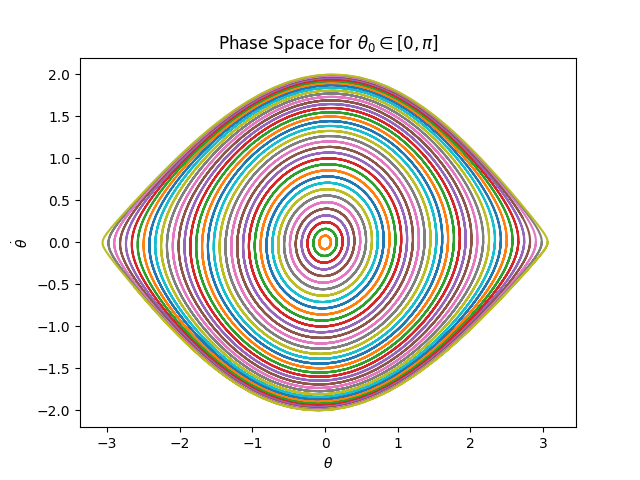
\includegraphics[scale=0.6]{../figures/phaseSpace.png}
	\caption{Plots of trajectory $(\theta,\dot{\theta})$, for many values of $\theta_{0} \in [0,\pi]$}
	\label{phase}
\end{figure}

\begin{figure}[ht!]
	\centering
	\begin{minipage}[b]{0.4\textwidth}
		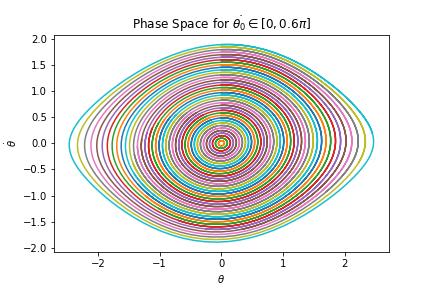
\includegraphics[scale=0.6]{../figures/phaseSpaceDot.png}
	\end{minipage}
	\hfill
	\begin{minipage}[b]{-- 0.4\textwidth}
		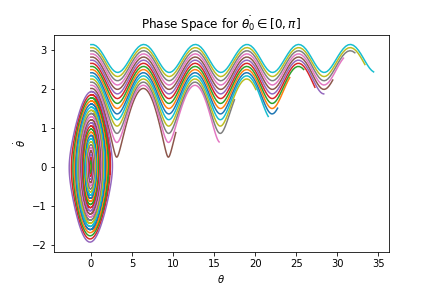
\includegraphics[scale=0.6]{../figures/phaseSpaceDot2.png}
	\end{minipage}
	\caption{Trajectory for various $\dot{\theta}$}
	\label{phaseDot}
\end{figure}
\end{problem}

%%%%%% 2B %%%%%%
\begin{problem}{2}
	\textbf{Phase space of linear pendulum} \\
	For the linear pendulum, the phase space trajectory remains elliptical for all values of $\theta_{0}$, as seen in figure \ref{phaseLin}

\begin{figure}[h!]
\centering
  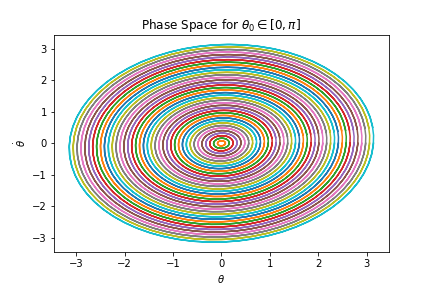
\includegraphics[scale=0.6]{../figures/phaseSpaceLinear.png}
  \caption{Plots of linearized trajectory $(\theta,\dot{\theta})$, for many values of $\theta_{0} \in [0,\pi]$}
  \label{phaseLin}
\end{figure}
\end{problem}

%%%%%% 3B %%%%%%
\begin{problem}{3}
	\textbf{Pendulum with driving force, $\gamma k^{2}cos(\omega t)$} \\
	If a periodic driving force with $\omega = k$ is added, the frequency stays the same, but the ampltude varies periodically, as seen in figure \ref{driving}. 
\begin{figure}[h!]
	\centering
  	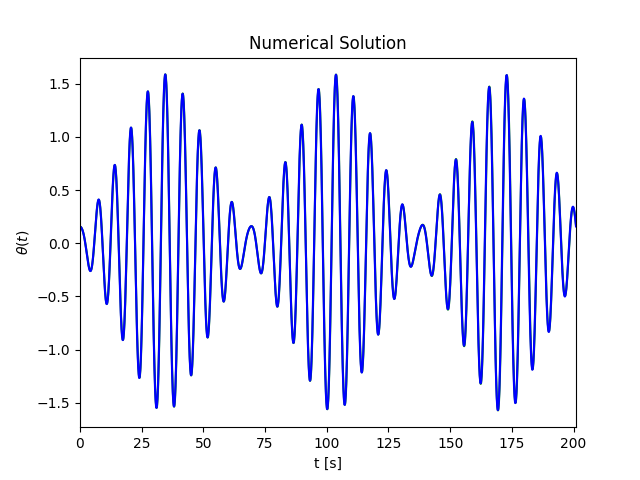
\includegraphics[scale=0.6]{../figures/drivingForce.png}
 	\caption{Solution for driven undamped pendulum}
  	\label{driving}
\end{figure}
\end{problem}

%%%%%% 4B %%%%%%
\begin{problem}{4}
	\textbf{Exploration of driven system} \\ Figure \ref{driving2} shows how the
  trajectories vary with $\gamma$. The upper two panes identify values of
  $\gamma$ that makes the pendulum display periodic behavior: for small
  $\gamma$, e.g. $0.0$, $0.14$, and $0.28$, the pendulum's motion is not
  affected much and retains the same period; when $\gamma = 1.43$, the pendulum
  exhibits period doubling as shown by the red phase space trajectory. The
  lower two panes show chaotic behavior under different values of $\gamma$. 

\begin{figure}[ht!]
	\centering
	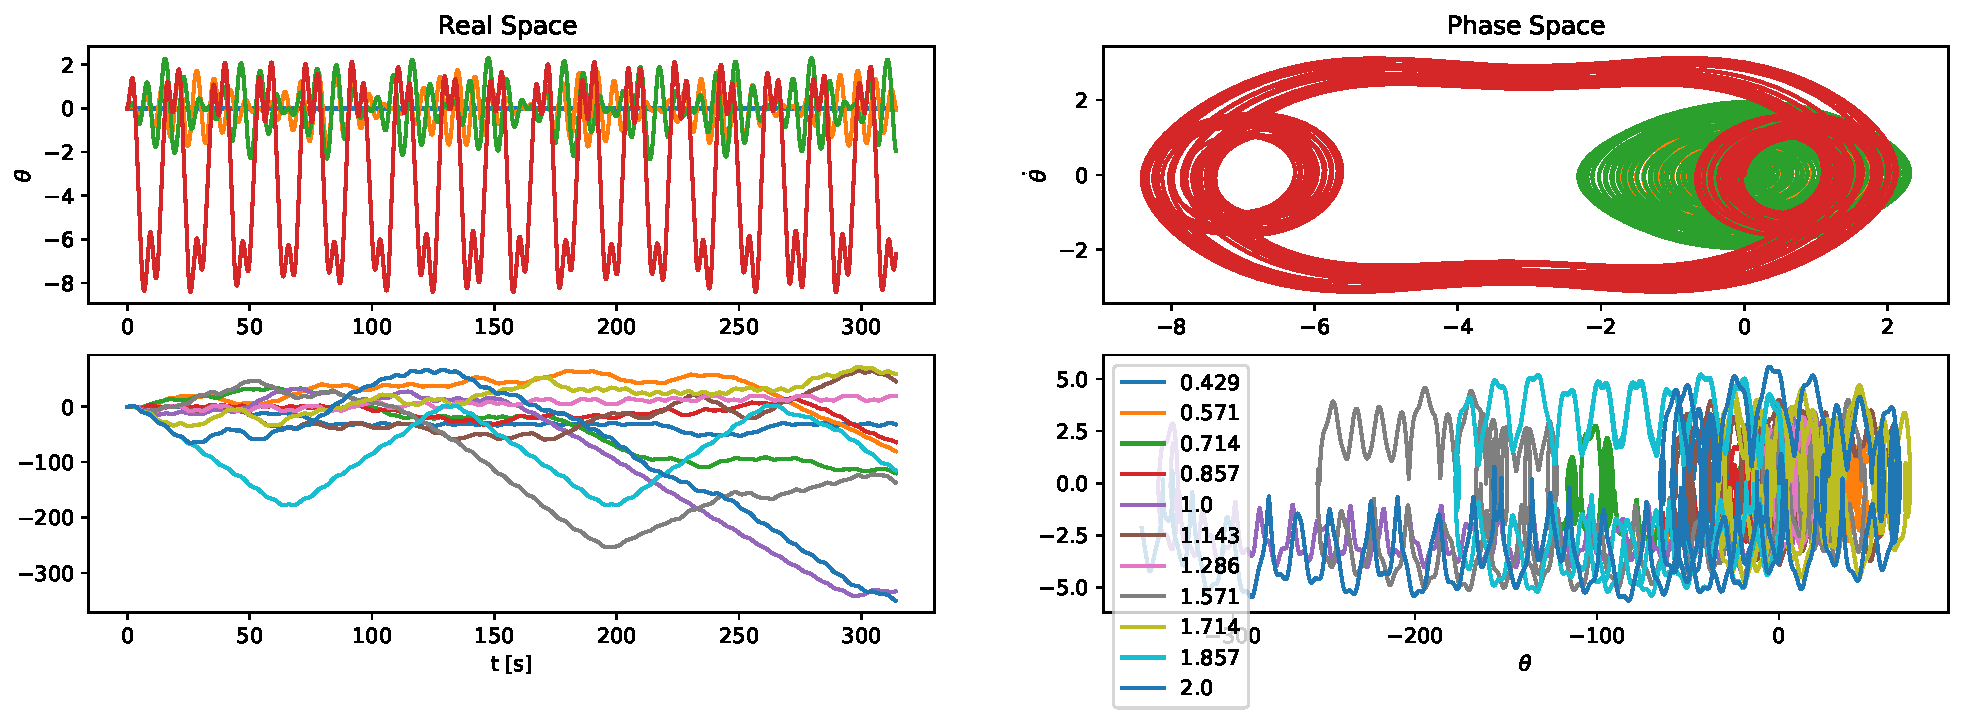
\includegraphics[scale=0.5]{../figures/driving2.pdf}
	\caption{Trajectories for undamped driven pendulum for $\gamma \in [0,2]$}
	\label{driving2}
\end{figure}
\end{problem}

%%%%%% 5B %%%%%%
\begin{problem}{5}
	\textbf{Identifying $(\theta_{0},\gamma)$ for which the motion diverges} \\

	Figure \ref{diverge} shows the phase plot for $(\theta_{0},\gamma)$ for $\theta_{0} \in [0,\pi]$, and $\gamma \in [0,6]$, after a time interval of $8\pi$ seconds.  The white regions indicate values for which the motion remained periodic. The blue regions indicate values for which the motion diverged.  The darker the color, the greater the value of $\theta$ at the end of the time interval.
\begin{figure}[h!]
	\centering
  	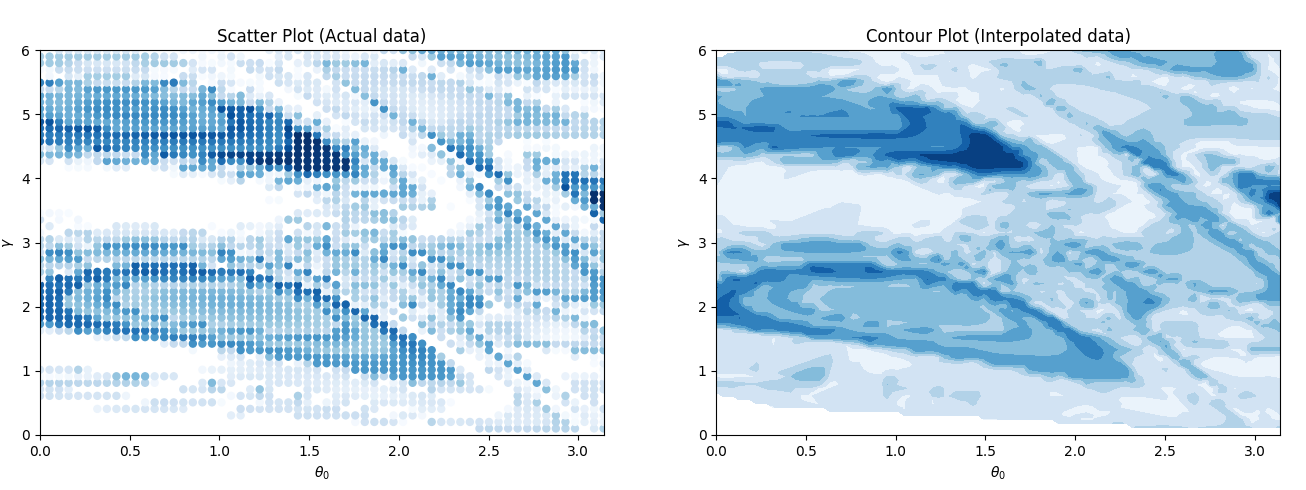
\includegraphics[scale=0.5]{../figures/diverge2.png}
 	\caption{Phase plot for $(\theta_{0},\gamma)$. On the left is the actual data that was calculated, and on the right is an interpolated contour plot.}
  	\label{diverge}
\end{figure}
\end{problem}

%%%%%% 6B %%%%%%
\begin{problem}{6}
	\textbf{Driven pendulum with damping} $\ddot{\theta}+2\beta\dot{\theta}+k^{2}sin\theta=\gamma k^{2}cos(\omega t)$ \\

As $\gamma$ increases, the pendulum transitions to chaos, as seen in figure \ref{damped}.  This transition is known as \textit{period doubling}, which is becomes apparent from observing the plots.  As $\gamma$ increases, some trajectories diverge and become nonperiodic, while some trajectories remain stable and periodic, with a period twice as long as before. Figure \ref{damped} only shows trajectories that remained periodic.

\begin{figure}[h!]
	\centering
  	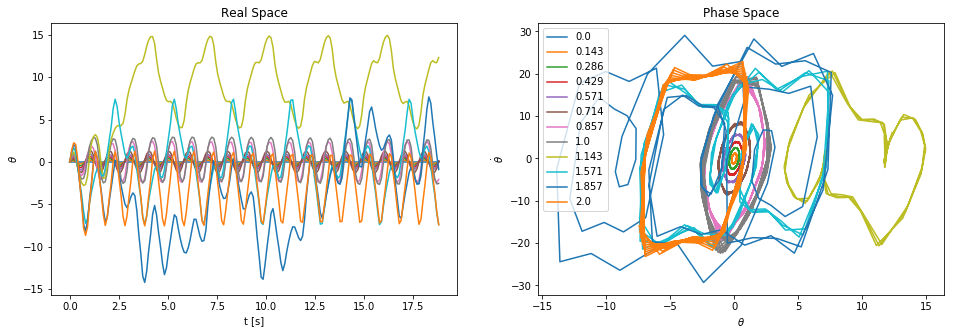
\includegraphics[scale=0.5]{../figures/dampedDriven.png}
 	\caption{Plots of driven damped pendulum for trajectory various values of $\gamma \in [0,2]$}
  	\label{damped}
\end{figure}

\end{problem}

%%%%%% 7B %%%%%%
\begin{problem}{7}
\textbf{Fourier analysis}

By taking the fourier transform of a periodic trajectory, we can determine the relative contribution of the various frequencies that make up the trajectory.  Figure \ref{fourier} shows the fast fourier transform of the trajectory that is colored yellow in figure \ref{damped}. Each spike corresponds to a frequency that is present in the trajectory, and the sizes of the spikes correspond to the amplitude of that frequency. 

\begin{figure}[h!]
	\centering
  	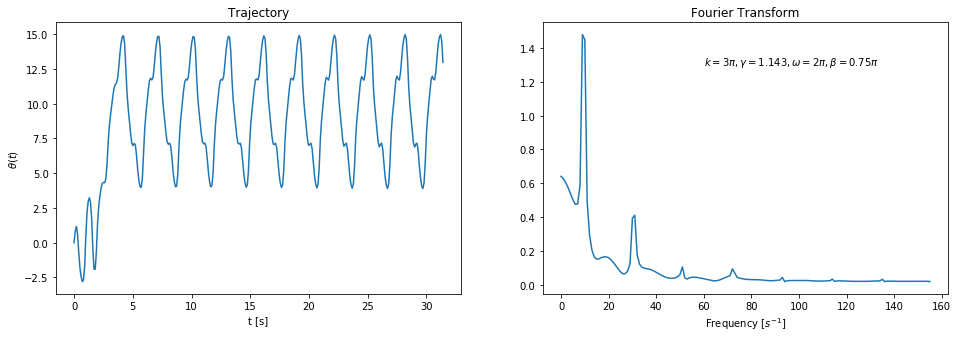
\includegraphics[scale=0.5]{../figures/fourier.png}
 	\caption{Fourier transform of damped driven pendulum with the parameters shown}
  	\label{fourier}
\end{figure}
\end{problem}
